% !TEX TS-program = pdflatex
% !TEX encoding = UTF-8 Unicode

\documentclass[12pt, a4paper]{article}
\usepackage[utf8]{inputenc}
\usepackage[T1]{fontenc}
\usepackage{helvet}
\usepackage{graphicx}
\usepackage{geometry}
\geometry{a4paper, landscape, margin=1.5cm}
\renewcommand{\familydefault}{\sfdefault}
\pagestyle{empty}

\begin{document}

% First side
\begin{minipage}[t][0.48\textheight][c]{\textwidth}
    \centering
    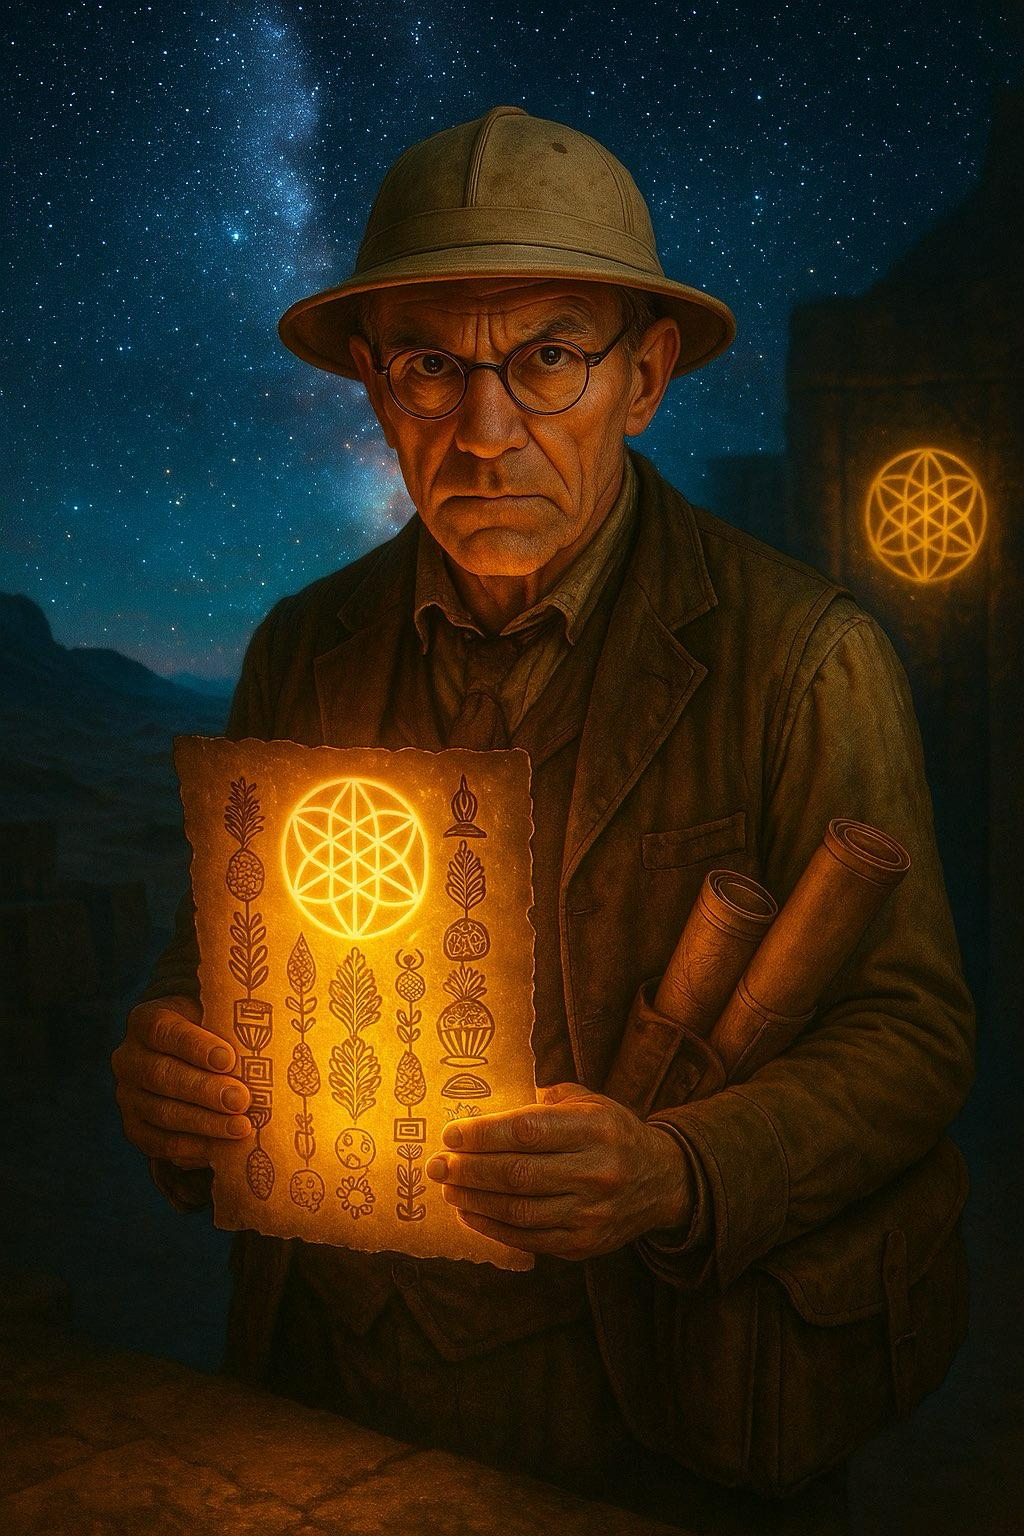
\includegraphics[height=6cm,keepaspectratio]{Voss.jpg} \\
    \vspace{1cm}
    {\fontsize{40}{48}\selectfont Dr. Alaric Voss} \\
    \vspace{0.5cm}
    {\Large\itshape "It's not a conspiracy if you're right!"}
\end{minipage}

\vfill

% Second side (for the other side of the tent)
\begin{minipage}[b][0.48\textheight][c]{\textwidth}
    \centering
    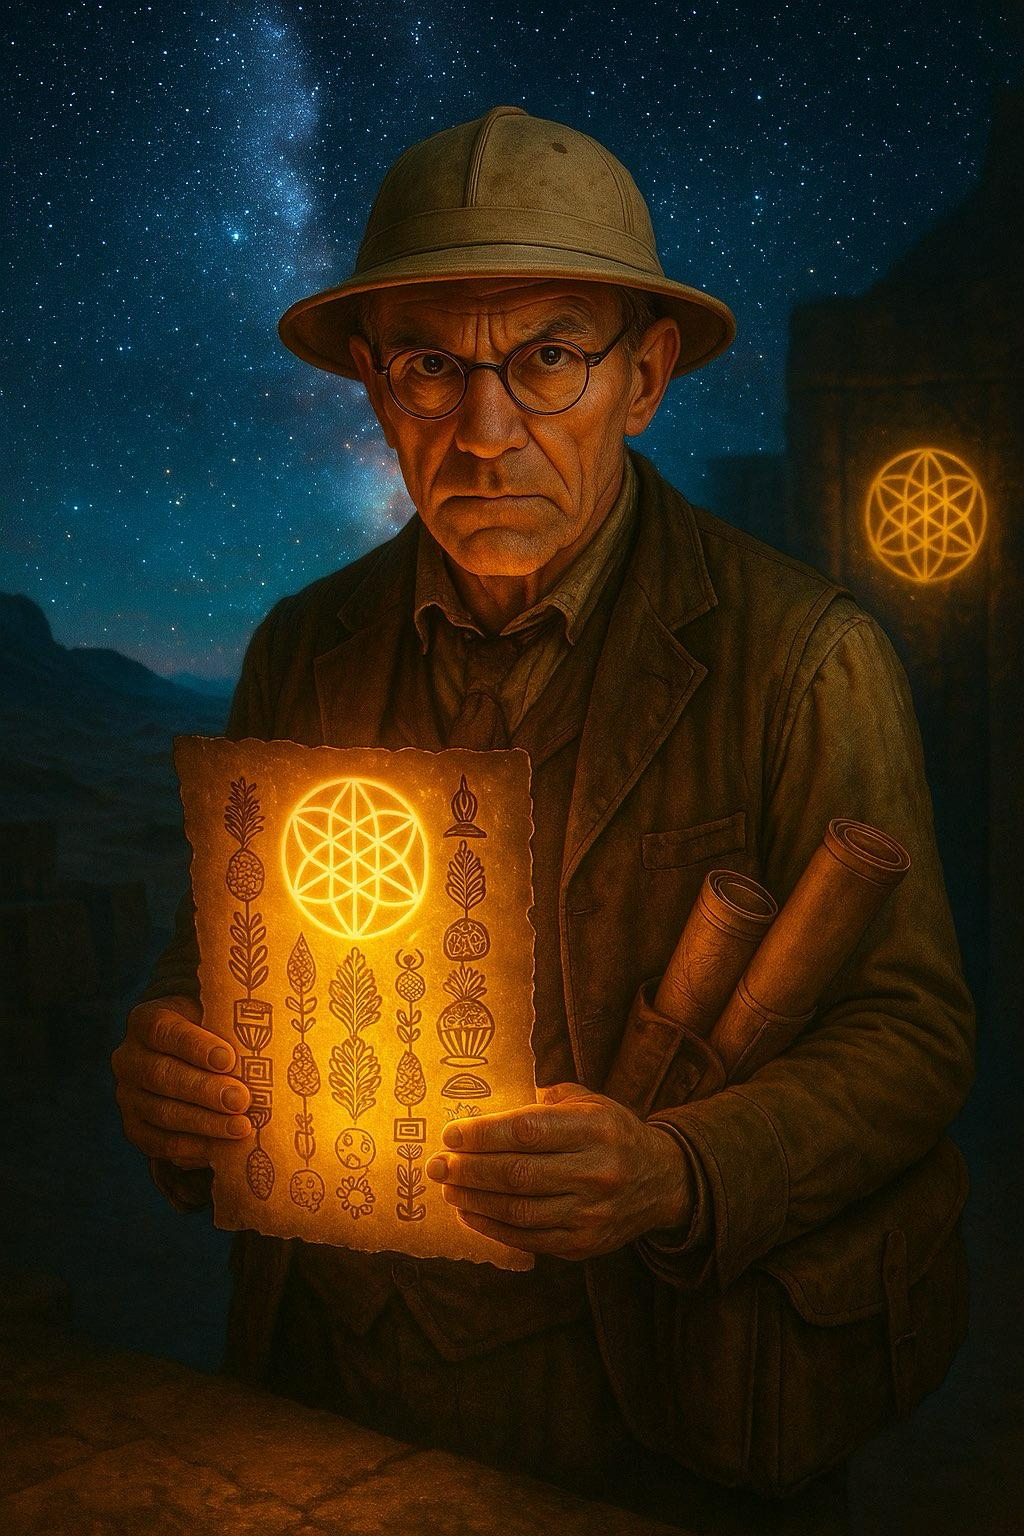
\includegraphics[height=6cm,keepaspectratio]{Voss.jpg} \\
    \vspace{1cm}
    {\fontsize{40}{48}\selectfont Dr. Alaric Voss} \\
    \vspace{0.5cm}
    {\Large\itshape "It's not a conspiracy if you're right!"}
\end{minipage}

\end{document} 